\chapter{ทฤษฎีที่เกี่ยวข้อง}
ในบทนี้จะอธิบายถึงองค์ความรู้และทฤษฎีต่างๆ ที่จำเป็นต่อการพัฒนาแอปพลิเคชั่นและเว็บเซอร์วิส โดยประกอบด้วยเนื้อหาดังต่อไปนี้
\begin{itemize}[label={--}]
	\item ความรู้พื้นฐานเกี่ยวกับ Ionic Framework
	\item ความรู้พื้นฐานเกี่ยวกับ Docker
	\item ความรู้พื้นฐานเกี่ยวกับ HTTP Protocol
	\item ความรู้พื้นฐานเกี่ยวกับ RESTful API
	\item การทำ Authentication ด้วย JSON Web Token
	\item ความรู้พื้นฐานเกี่ยวกับ OpenCV
	\item การหาขนาดของยาด้วยการใช้วัถตุอ้างอิง
	\item เครื่องมือที่ใช้ในการพัฒนา
\end{itemize}

\section{ความรู้พื้นฐานเกี่ยวกับ Ionic Framework}
	Ionic Framework [16] เป็นเครื่องมือที่ใช้ในการพัฒนา Mobile Application แบบ Hybrid Mobile Application ที่สามารถทำงานได้หลาย Platforms ทั้งระบบปฏิบัติการไอโอเอสและระบบปฏิบัติการแอนดรอยด์ โดยจะใช้เทคโนโลยีในการพัฒนาคือ HTML CSS และ JavaScript โดยเป็นภาษาหลักในการใช้พัฒนาแอพพลิเคชันเนื่องจากใช้แกนหลังเป็น AngularJS และมีการใช้งาน Command-line interface (CLI) สำหรับจัดการดูแลบริการต่างๆ ใน เช่น การสร้างหน้า การติดตั้ง เป็นต้น ผู้พัฒนาพัฒนาแอปพลิเคชันค้นหายาเพื่อคุณด้วย Ionic Framework เนื่องจาก Ionic Framework สามารถพัฒนาได้หลาย Platforms และใช้เทคโนโลยีพื้นฐานของการพัฒนาเว็บไซต์ คือ HTML CSS และ JavaScript 

	\begin{figure}[H]
		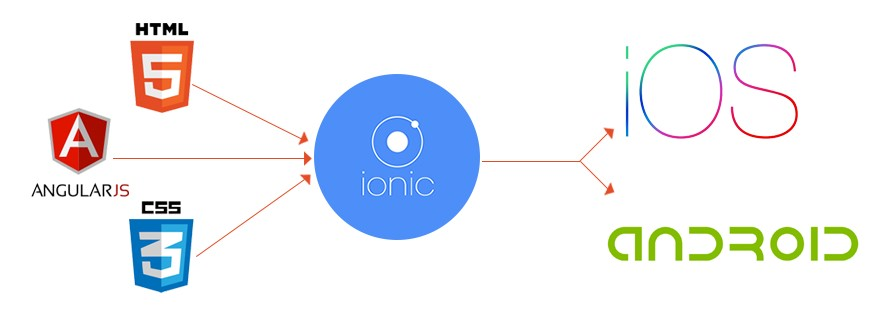
\includegraphics[width=\columnwidth]{Figures/2/ionic-structure}
		\caption{โครงสร้างของ Ionic Framework}
		\label{Fig:ionic-structure}
	\end{figure}
	
	\subsection{รายละเอียดของ Cordova}
		Cordova ถูกพัฒนาจาก Nitobi ในปี ค.ศ.2009 เป็น Open Source ที่ช่วยให้เทคโนโลยีเว็บสามารถใช้งานกับมือถือได้ ซึ่งก่อนหน้ามีชื่อว่า “PhoneGap” และ Cordova เป็นตัวจัดการเทคโนโลยีเว็บให้เข้าถึงการทำงานของระบบปฏิบัติการ เช่น การถ่ายรูป การเรียกไฟล์จากตัวเครื่อง จีพีเอส เป็นต้น ด้วยการทำงานผ่านไลบรารี่ (Library) ซึ่งสามารถใช้ได้ทุกระบบปฏิบัติการทั้ง Window Phone, Blackberry, IOS หรือ Android 

		\begin{figure}[H]
			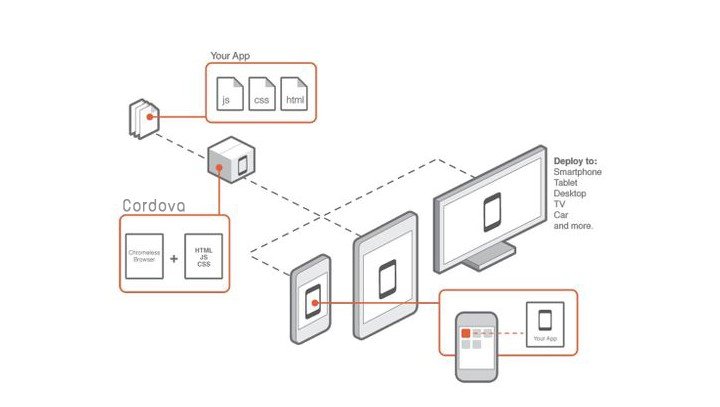
\includegraphics[width=\columnwidth]{Figures/2/cordova-structrue}
			\caption{โครงสร้างของ Cordova}
			\label{Fig:cordova-structrue}
		\end{figure}

	\subsection{Hybrid Mobile Application }
		Ionic Framework เป็นแอปพลิเคชั่นประเภท Hybrid Mobile เป็นการเขียนแอปพลิเคชันระหว่าง Native Application [11] และ Web Application [12] เพื่อแก้ไขปัญหาในการทำงานซ้ำซ้อนระหว่างระบบปฏิบัติการ ซึ่งการเขียนแอพพลิเคชั่นสามารถใช้งานได้กับทุกระบบปฏิบัติการ และยังสามารถเรียกใช้งานทรัพยากรของระบบปฏิบัติการของโทรศัพท์สมาร์ทโฟนนั้นได้อย่างอิสระ

	\subsection{Lifecycle events }
		การเปลี่ยนหน้าเพจของ Ionic framework จะเป็นการสแตก (Stack) ของหน้าเพจ มีคำสั่ง pop สำหรับดึงหน้าเพจออกจากสแตกและคำสั่ง push สำหรับซ้อนทับหน้าเพจใหม่เข้ามาในสแตก
		
		Lifecycle events [10] จะเกิดขึ้นในระหว่างการเปลี่ยนหน้าเพจ 
		การแสดงเพิ่มเข้ามาและการปิดหรือลบออกไปของ Component ที่มีรูปแบบการใช้งานคล้ายเพจ 
		ในบางครั้งการกำหนดการทำงานแทรกเข้าไปในเพจ ดังต่อไปนี้

		\begin{enumerate}
			\item ionViewDidLoad: เริ่มทำงานเมื่อโหลดหน้าเพจและถูกเก็บข้อมูลในหน่วยความจำ กิจกรรมนี้จะไม่เกิดขึ้นเมื่อหน้าเพจมีการแคช (Cache) เกิดขึ้น
			\item ionViewWillEnter: เริ่มทำงานเมื่อหน้าเพจถูกเรียกขึ้นมาแสดงและกลายเป็นหน้าเพจที่ใช้งานอยู่
			\item ionViewDidEnter: เริ่มทำงานเมื่อหน้าเพจที่ใช้งานอยู่ถูกเรียกมาอย่างสมบูรณ์ กิจกรรมนี้จะไม่เกิดขึ้นเมื่อหน้าเพจมีการแคชเกิดขึ้น
			\item ionViewWillLeave: เริ่มทำงานเมื่อกำลังจะออกจากหน้าเพจและไม่ใช่หน้าเพจที่ใช้งานอยู่
			\item ionViewDidLeave: เริ่มทำงานเมื่อออกจากหน้าเพจเสร็จสิ้นแล้วและไม่ใช่หน้าเพจที่ใช้งานอยู่
			\item ionViewWillUnload: เริ่มทำงานเมื่อหน้าเพจนั้นถูกทำลายหรือถูกลบหน้าเพจออกไป
			\item ionViewCanEnter: เริ่มการทำงานก่อนจะโหลดหน้าเพจ ใช้สำหรับกำหนดสิทธิการเข้าไปยังหน้าเพจ
			\item ionViewCanLeave: เริ่มการทำงานก่อนมีการออกจากหน้าเพจ ใช้สำหรับกำหนดเงื่อนไขในการออกจากหน้าเพจ
		\end{enumerate}

	\subsection{ข้อดีและข้อเสียของ Ionic Framework}
		\begin{enumerate}
			\item ข้อดีของ Ionic Framework
			\begin{itemize}
				\item สามารถทำงานใช้งานได้หลายระบบปฏิบัติการ
				\item มีส่วนติดต่อผู้ใช้งาน (User Interface) ที่ถูกออกแบบมาสวยงาม 
				\item ใช้เทคโนโลยี HTML CSS และ JavaScript ที่ได้รับการยอมรับและใช้งานอย่างแพร่หลาย	
			\end{itemize}
			\item ข้อเสียของ Ionic Framwork
				\begin{itemize}
					\item มีข้อจำกัดการทำงานใน WebView [6] ของระบบปฏิบัติการแอนดรอยด์ 4.0 ในการเล่น Animation รวมถึงการทำงานของ JavaScript ค่อนข้างช้า
				\end{itemize}
		\end{enumerate}

\section{ความรู้พื้นฐานเกี่ยวกับภาษา TypeScript}
	TypeScript เป็นภาษาโปรแกรมที่พัฒนาโดย Microsoft



\section{ความรู้พื้นฐานเกี่ยวกับ Docker }
	Docker [9] เป็นซอฟแวร์ Open-source สำหรับสร้างแพ็จเกจของ application ที่เก็บรวมเข้าไว้ด้วยกันใน Container 
	ที่มีการทำงานในลักษณะจำลองสภาพแวดล้อมขึ้นมาบนเครื่องเซิฟเวอร์ 
	เพื่อใช้ในการเริ่มการทำงานของเซอร์วิสที่ต้องการ 
	มีการทำงานคล้ายคลึงกับ Virtual Machine 
	แต่มีข้อแตกต่างกันในการจำลองสภาพแวดล้อมทั้ง OS 
	เพื่อใช้งาน แต่สำหรับ Docker จะใช้ Container ในการจำลองสภาพแวดล้อมขึ้น 
	เพื่อใช้งานสำหรับเซอร์วิสที่ต้องการใช้งานเท่านั้น 
	โดยไม่มีส่วนของ OS เข้าไปเกี่ยวข้องเหมือนกับ Virtual Machine แสดงดังรูปที่ \ref{Fig:containers_vs_VM}
	
	ในการติดตั้งเว็บเซอร์วิสที่เครื่องเซิฟเวอร์ที่มีสภาพแวดล้อมไม่เหมือนกับเครื่องที่ใช้พัฒนา 
	จำเป็นจะต้องติดตั้งส่วนเสริมเพิ่มเติมเข้ามาในเครื่องเซิฟเวอร์อีก และเพื่อป้องกันปัญหานี้ 
	ผู้พัฒนาได้พัฒนาเว็บเซอร์วิสของแอปพลิเคค้นหายาเพื่อคุณไว้ใน 
	Docker image สำหรับพร้อมติดตั้งด้วย Docker Engine  

	\begin{figure}
		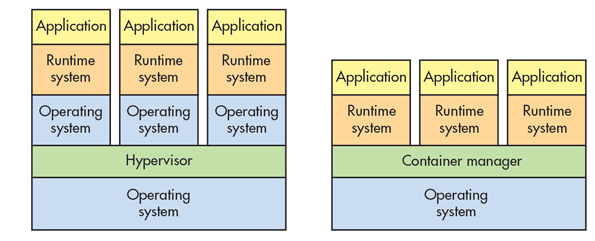
\includegraphics[width=\columnwidth]{Figures/2/containers_vs_VM}
		\caption{ความแตกต่างสถาปัตยกรรมระหว่าง Containers และ Virtual Machines}
		\label{Fig:containers_vs_VM}
	\end{figure}

	\subsection{รายละเอียดของ Docker Concepts}
		\begin{enumerate}
			\item Images เป็นเหมือนกับตัวต้นแบบของ container ภายในประกอบด้วย application ที่มีการติดตั้งเพื่อใช้งานสำหรับเซอร์วิส มีการกำหนดการตั้งค่าไว้เรียบร้อย และนำมาสร้างเป็น docker images เก็บไว้บน docker registry เพื่อนำไปใช้งาน
			\item Container ถูกสร้างมาจาก images และเมื่อสร้างขึ้นมาจะเป็นการเริ่มทำงานของเซอร์วิส ซึ่งภายใน container แต่ละตัวจะมีการใช้งาน RAM CPU และไฟล์ config เป็นต้น เปรียบเสมือนเป็นเครื่องเซิฟเวอร์ผู้ใช้งานสามารถควบคุมและจัดการกับ binaries, dependencies ทั้งหมดได้ใน container
			\item Registries and Repositories เป็นคลาวด์เซิร์ฟเวอร์สำหรับเก็บ image ไว้บน DockerHub [15] และภายใน registry จะมี repositorites ที่เอาไว้จัดเก็บ image ที่อยู่ใน registry
		\end{enumerate}

	\subsection{ข้อดีของ Docker}
		\begin{enumerate}
			\item สามารถใช้งานได้บน Linux Mac และ Windows
			\item มีขนาดข้อมูลเล็กและการติดตั้งได้อย่างเร็วรวด เพราะไม่มีส่วน OS
			\item มีความต้องการในการใช้ CPU RAM และพื้นที่น้อยกว่า Virtual Machine
			\item ลดปัญหาสภาพแวดล้อมที่ต่างกัน ระหว่างติดตั้งที่เครื่องเซิฟเวอร์
			\item ผู้ใช้งานสามารถ pull image จาก docker registry ที่มีการสร้างไว้ให้แล้วมาใช้งาน 
		\end{enumerate}
	\subsection{คำสั่งเบื้องต้น}
		มีคำสั่งเบื้องต้นดังต่อไปนี้
		\begin{enumerate}
			\item docker images แสดงรายการรายละเอียด images ทั้งหมดบนเครื่องผู้ใช้งาน
			\item docker pull คำสั่งดึง images จาก registry มาไว้ที่เครื่องผู้ใช้งาน
			\item docker ps แสดงรายการรายละเอียดของ container ที่กำลังทำงานอยู่ทั้งหมด
			\item docker stop CONTAINER ID คำสั่งหยุดการทำงานของ container 
			\item docker start CONTAINER ID คำสั่งเริ่มการทำงานของ container 
			\item docker rm CONTAINER ID คำสั่งลบ container
			\item docker logs CONTAINER ID คำสั่งเพื่อดูข้อมูลการทำงานของ container
			\item docker run IMAGES NAME ใช้ในการสร้าง container ใหม่ ในกรณีที่ไม่มี images นั้นๆ บนเครื่องผู้ใช้งาน docker จะ pull images มาไว้ที่เครื่องผู้ใช้งานโดยอัตโนมัติ
		\end{enumerate}
	
	\subsection{การใช้งาน Docker ใน Ubuntu}
		การใช้งาน Docker ใน Ubuntu [17] สามารถอธิบายได้ดังรูปที่ \ref{Fig:UsingDocker} ดังต่อไปนี้
		\begin{itemize}[label={--}]
			\item บรรทัดที่ 1 – 2 เป็นการติดตั้ง Docker สามารถเรียกใช้ผ่าน Command line
			\item บรรทัดที่ 3 ทดสอบการทำงานของ Docker ด้วยการเรียกใช้งาน Image ที่ชื่อ “hello-world”
			\item บรรทัดที่ 4 – 8  ถ้าที่เครื่องผู้ใช้งานไม่มี image นั้น Docker จะทำการดาวโหลดจาก Docker Hub มาที่เครื่องผู้ใช้งาน 
			\item บรรทัดที่ 9 Docker สามารถทำงานได้ตามปกติ และเรียกใช้งาน Image hello-world ได้สำเร็จ
		\end{itemize}

		\begin{figure}[H]
			{\setstretch{1.0}\begin{lstlisting}
sudo apt - get update 
sudo apt - get install - y docker - ce   
docker   run hello-world   
Unable  to  find  image  'hello-world:latest'  
locally  latest:  Pulling  from  library  /  hello  -  world  
78445 dd45222: Pull complete Digest: sha256: c5515758d4c5e1e838e9cd307f6c6a0d 620b5e07e6f927b07d05f6d12a1ac8d7  
Status: Downloaded newer image  
for  hello  -  world:  latest  
Hello   from   Docker!This   message   shows   that   your   installation   appears   to   be   working   correctly. 
			\end{lstlisting}}
			\caption{คำสั่งในการใช้งาน Docker}
			\label{Fig:UsingDocker}
		\end{figure}
		

\section{ความรู้พื้นฐานเกี่ยวกับ HTTP Protocol}
	HTTP (Hypertext Transfer Protocol) เป็นโปรโตรคอลที่อยู่ในส่วนของ Application Layer 
	และเป็นโปรโตรคอลสื่อสารสำหรับการแลกเปลี่ยนสารสนเทศอินเทอร์เน็ตของ World Wide Web (WWW) 
	ซึ่งมีโครงสร้างเป็นตัวอักษรและตัวเลข (Text) เรียกว่า ทรัพยากร (Resource) 
	โดยทรัพยากรเป็นข้อมูลต่างๆ เช่น HTML ไฟล์ รูปภาพ และวิดิโอ เป็นต้น
	
	แอปพลิเคชันค้นหายาเพื่อคุณอาศัย HTTP ในการสือสารกับเว็บเซอร์วิส โดยใช้ HTTP Method สำหรับร้องขอทรัพยากร (HTTP Request) จากเว็บเซอร์วิสและคืนทรัพยากร (HTTP Response) จากเว็บเซอร์วิสมายังเครื่องผู้ใช้งาน 

	\subsection{HTTP Method}
		HTTP ได้กำหนดคำสั่งร้องขอไว้ทั้งหมด 8 คำสั่ง แสดงการกระทำที่ต้องการ เพื่อที่จะดำเนินการกับทรัพยากรที่ถูกระบุ ดังต่อไปนี้

		\begin{enumerate}
			\item HEAD ร้องขอการตอบรับจากทรัพยากรที่ระบุ คล้ายกับ GET แต่จะไม่มีส่วนเนื้อหาที่ร้องขอกลับมา คำสั่งนี้ใช้ประโยชน์ในการตรวจสอบข้อมูลส่วนห้วของการตอบรับ โดยไม่จำเป็นต้องส่งเนื้อหาเต็มมาทั้งหมด
			\item GET ร้องขอการนำเสนอจากทรัพยากรที่ระบุและมีส่วนของเนื้อหาที่ร้องขอ
			\item POST ส่งข้อมูลไปยังทรัพยากรที่ระบุเพื่อให้นำไปประมวล
			\item PUT อัปโหลดการนำเสนอของทรัพยากรที่ระบุ
			\item DELETE ลบทรัพยากรที่ระบุ
			\item TRACE ส่งข้อมูลร้องขอกลับมา เครื่องลูกข่ายจะเห็นว่ามีข้อมูลที่สื่อกลางเพิ่มหรือเปลี่ยนแปลงข้อความร้องขอก่อนไปถึงทรัพยากรปลายทาง
			\item OPTIONS คืนค่าเป็นรายชื่อคำสั่ง HTTP ที่เครื่องแม่ข่ายนั้นรองรับสำหรับทรัพยากรที่ระบุ
			\item CONNECT แปลงการเชื่อมต่อของการร้องขอไปเป็น TCP/IP [14]
		\end{enumerate}

	\subsection{รายละเอียดของ HTTP Request}
		รูปแบบโครงสร้างของ HTTP Request เป็นการข้อมูลโดยผู้ใช้งานไปยังเซิฟเวอร์เพื่อให้ส่งข้อมูลตอบกลับมาที่ผู้ใช้งานแสดงดังรูปที่ \ref{Fig:HTTP-request-structrue} และรายละเอียดใน HTTP Request มีดังนี้
	\subsection{รายละเอียดของ HTTP Response}
		\begin{enumerate}
			\item <VERB> เป็นส่วนของ HTTP method 
			\item <URL> เป็นตำแหน่งของสถานที่ข้อมูลที่ต้องการให้ระบบทำงาน
			\item <HTTP Version> เป็นเวอร์ชันของ HTTP
			\item <Request Header> เป็นส่วนของ Metadata ที่ใช้เก็บค่า key-value ของ Header เพื่อบอกข้อมูลผู้ส่ง
			\item <Request Body> เป็นส่วนข้อมูล Content ใน REST
		\end{enumerate}
		\begin{figure}
			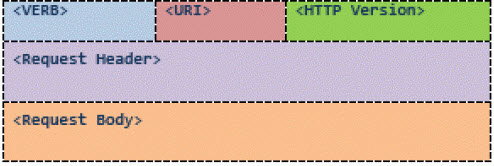
\includegraphics[width=\columnwidth]{Figures/2/HTTP-request-structrue}
			\caption{รูปแบบโครงสร้างของ HTTP Request}
			\label{Fig:HTTP-request-structrue}
		\end{figure}

	\subsection{รายละเอียดของ HTTP Response}
		รูปแบบโครงสร้างของ HTTP Response คือการส่งข้อมูลที่ทางเซิฟเวอร์ตอบรับกลับไปยังผู้ใช้งานตามที่ได้ขอมาแสดงดังรูปที่ \ref{Fig:HTTP-response-structrue} และรายละเอียดใน HTTP Response มีดังนี้

		\begin{enumerate}
			\item <HTTP Version> เป็นเวอร์ชันของ HTTP
			\item <Response Code> เป็นผลลัพธ์การทำงานในระบบ HTTP เป็นตัวเลข 3 หลัก เช่น 2XX การร้องขอสำเร็จ, 3XX การเปลี่ยนทาง, 4XX ความผิดพลาดจากเครื่องผู้ใช้งาน, 5XX ความผิดพลาดจากเครื่องเซิฟเวอร์
			\item <Request Body> เป็นส่วนข้อมูลผลลัพธ์ Content ใน REST ที่เซิฟเวอร์ตอบกลับมาที่ผู้ใช้งาน
		\end{enumerate}
		\begin{figure}
			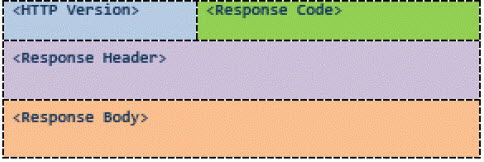
\includegraphics[width=\columnwidth]{Figures/2/HTTP-response-structrue}
			\caption{รูปแบบโครงสร้างของ HTTP response}
			\label{Fig:HTTP-response-structrue}
		\end{figure}

\section{ความรู้พื้นฐานเกี่ยวกับ RESTful API}
	REST (Representational state transfer) คือการสร้างเว็บเซอร์วิสชนิดหนึ่งที่อาศัย HTTP Method GET, POST, PUT และ DELETE ในการทำงาน ใช้หลักการแบบ stateless คือไม่มีการใช้งาน session และส่งผลกลับมาในรูปแบบของ JSON หรือ XML มีขนาดข้อมูลที่เล็ก สามารถส่งผลให้สามารถรับส่งข้อมูลไปมาข้าม Platform ได้อย่างสะดวก เนื่องจากเป็นการเรียกใช้งานผ่าน HTTP Protocol ที่ใช้ในการเรียกเว็บไซต์ จึงเป็นที่นิยม และแอปพลิเคชันค้นหายาเพื่อคุณกับเว็บเซอร์วิสติดต่อสื่อสารผ่าน HTTP โดยใช้ HTTP method ในการร้องขอทรัพยากรจากเว็บเซอร์วิสและส่งทรัพยากรกลับมาที่แอปพลิเคชันในรูปแบบของ JSON ดังแสดงในรูปที่ 
	\ref{fig:format-JSON}  

	\begin{figure}
		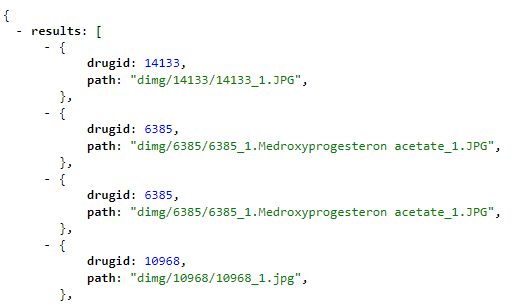
\includegraphics[width=\columnwidth]{Figures/2/format-JSON}
		\caption{ตัวอย่างรูปแบบของ JSON}
		\label{fig:format-JSON}
	\end{figure}

\section{การทำ Authentication ด้วย JSON Web Token }
	\subsection{การพิสูจน์ตัวตน (Authentication)}
		ในบางแอพพลิเคชั่นจะสามารถใช้งานได้จำเป็นต้องรู้จักผู้ใช้งานที่กำลังใช้งานอยู่ ซึ่งระบบที่ทำหน้าที่ในการตรวจสอบ เรียกว่า “Authentication” 
	
		ผู้พัฒนาได้พัฒนาการพิสูจน์ตัวตนก่อนใช้งานเว็บเซอร์วิสด้วย JSON Web Token [1] เพื่อป้องการเข้าถึงข้อมูลจากผู้ที่ไม่พึ่งประสงค์ โดยการร้องขอทรัพยากรไปยังเว็บเซอร์วิสจากแอปพลิเคชันค้นหายาเพื่อคุณ จะฝั่ง JSON Web Token ไว้ใน Header ของ HTTP Requset เพื่อไว้สำหรับการพิสูจน์ตัวตนของเว็บเซอร์วิส และรายละเอียดของ JSON Web Token มีดังนี้ 
	
	\subsection{รายละเอียดของ JSON Web Token (JWT) }
		JSON Web Token เป็นมาตรฐานเปิด (RFC 7519) ที่เข้ามาแก้ปัญหาการส่งข้อมูลอย่างปลอดภัยระหว่างแอพพลิเคชั่นและเว็บเซอร์วิส โดยถูกออกแบบให้มีขนาดที่กระทัดรัด (Compact) และเก็บข้อมูลภายในตัว (Self-contained) JWT เป็น Token หรือ ชุดตัวอักษร โดยมีโครงสร้างแบ่งออกเป็น 3 ส่วน ได้แก่
		\begin{enumerate}
			\item Header สำหรับเก็บประเภทการเข้ารหัสของโทเคน 
			\item Payload สำหรับเก็บข้อมูล
			\item Signature ส่วน Digital Signed ซึ่งเหมือนกับลายเซ็นทิ้งท้ายไว้ตรวจสอบว่าเป็นโทเคนที่ถูกสร้างอย่างถูกต้องหรือไม่ถูกต้อง และถ้าหากมีผู้เขียนแปลงข้อมูลของโทเคนจะทำให้การตรวจสอบ Signature ไม่ถูกต้อง 
		\end{enumerate}
		\begin{figure}
			
\includegraphics[width=\columnwidth]{Figures/2/JWT-structure}
			\caption{ตัวอย่างรูปแบบของ JSON Web Token}
			\label{fig:JWT-structure}
		\end{figure}

	\subsection{การใช้งาน JSON Web Token}
	ผู้พัฒนาเลือกพัฒนา JWT ด้วย Node.js ที่มีแพ็กเกจรองรับการใช้งาน JWT
	\begin{enumerate}
		\item การสร้าง JSON Web Token
		จากรูปที่ \ref{Fig:SignJWT} สามารถอธิบายได้ดังนี้
		\begin{itemize}
			\item บรรทัดที่ 1 เรียกแพ็กเกจ jsonwebtoken มาเก็บที่ตัวแปร jwt
			\item บรรทัดที่ 2 เรียกใช้งานฟังก์ชัน sign สำหรับการสร้าง JSON WebToken โดยกำหนดให้ data คือ“foobar” คำลับ คือ “secret” และเวลาหมดอายุของ Token คือ 1 ชั่วโมง
		\end{itemize}
		\begin{figure}[H]
			{\setstretch{1.0}\begin{lstlisting}
var  jwt  =  require('jsonwebtoken');  
var  token  =  jwt.sign({  
	data: 'foobar'  
}, 'secret', {  
	expiresIn: '1h'  
});  
			\end{lstlisting}}
			\caption{ตัวอย่างการสร้าง JSON Web Token}
			\label{Fig:SignJWT}
		\end{figure}

		\item การตรวจสอบ JSON Web Token
			ในการตรวจสอบความถูกต้องของโทเคน คำลับในการสร้างและการตรวจสอบต้องเหมือนกัน 
			โทเคนจะต้องไม่หมดอายุและโทเคนจะต้องไม่ถูกเปลี่ยนตัวอักษร
			จากรูปที่ \ref{Fig:VerifyJWT} สามารถอธิบายได้ดังนี้
			\begin{itemize}
				\item บรรทัดที่ 1 เรียกใช้งานฟังก์ชัน verify สำหรับตรวจสอบความถูกต้องของ token โดยกำหนดคำลับ คือ ‘secret’ 
				\item บรรทัดที่ 2 เมื่อการตรวจสอบ token เสร็จแล้ว จะได้ผลลัพธ์ในตัวแปรชื่อว่า decoded ถ้าหากการตรวจสอบถูกต้องตัวแปร err จะมีค่าเป็น null และถ้าหากการตรวจสอบไม่ถูกต้องตัวแปร err มีค่าเป็นข้อความผิดพลาดจากการตรวจสอบ
			\end{itemize}
			\begin{figure}[H]
				{\setstretch{1.0}\begin{lstlisting}
jwt.verify(token,  'secret',  function(err,  decoded)  {  
	console.log(decoded)  
});  
				\end{lstlisting}}
				\caption{ตัวอย่างการตรวจสอบ JSON Web Token}
				\label{Fig:VerifyJWT}
			\end{figure}
	\end{enumerate}
	
	\subsection{ข้อดีและข้อเสียของ JWT}
		\begin{enumerate}
			\item ข้อดีของใช้งาน JWT สำหรับการ Authentication
			\begin{itemize}
				\item JWT สามารถใช้งานได้กับทุกภาษาที่รองรับข้อมูลแบบ JSON 
				\item สามารถส่ง JWT ผ่าน HTTP ใน Header POST และ URL ได้ง่าย รวดเร็ว
				\item มีความปลอดภัยในตัวของมันเอง 
			\end{itemize}
			\item ข้อเสียของใช้งาน JWT สำหรับการ Authentication 
			\begin{itemize}
				\item JWT สามารถเก็บข้อมูลในตัวเอง แต่ข้อมูลนั้นต้องเป็นข้อมูลที่สามารถเปิดเผยได้
				\item ถ้าหาก JWT ถูกขโมยไปใช้กับเว็บเซอร์วิส ก็จะสามารถทำ Authentication API ได้
				\item ข้อมูลที่ถูกเก็บไว้ใน JWT จะไม่สามารถถูกอัพเดทข้อมูลได้
			\end{itemize}
		\end{enumerate}
		
			
\section{ความรู้พื้นฐานเกี่ยวกับ OpenCV (Open Source Computer Vision) }
	OpenCV เป็นไลบรารี่ (Library) ที่รวบรวมฟังก์ชั่นสำหรับการประมวลผลภาพและคอมพิวเตอร์วิทัศนศาสตร์ไว้เป็นจำนวนมาก อยู่ภายใต้ใบอนุญาติ BSD ซึ่งสามารถใช้ได้ฟรีทั้งทางด้านการศึกษาและทางการค้า เนื่องจากนี้ยังมีการประยุกต์ใช้งาน OpenCV ในแบบต่างๆ ได้แก่ ระบบตรวจจับใบหน้า (Face Detection) การจดจำใบหน้า (Face Recognition) การติดตามวัถตุ (Object Tracking) การเรียนรู้ของเครื่อง (Machine Learning) เป็นต้น
	\subsection{การประมวลผลภาพ (Image Processing)}
	การประมวลผลภาพคือการนำรูปที่มีอยู่แล้ว หรือรูปที่รับเข้ามาจากอุปกรณ์ต่างๆ 
	หรือรูปที่มีอยู่มาประมวลผลเพื่อหาลักษณะเด่นบางประการของรูปที่มีอยู่ 
	หรืออาจจะเป็นการตีความหมายของภาพ รวมถึงการปรับคุณลักษณะของภาพให้เป็นไปตามต้องการ 
	โดยใช้กระบวนการทางคณิตศาสตร์
	
	การประมวลผลภาพแนวคิดทางคณิตศาสตร์ที่ใช้ในการประมวลผล Signal processing 
	มาทำการประยุกต์ใช้กับสัญญาณภาพ และภาพจะเก็บอยู่ในรูปของอาเรย์ (Array) 
	โดยกลุ่มของของอาเรย์กลุ่มหนึ่งจะเป็นค่าของภาพหนึ่งพิกเซล 
	เช่น ภาพแบบ RBG ใช้อาเรย์ 3 ช่องเพื่อเก็บค่าสีของ RBG ในหนึ่งพิกเซล รูปแบบการจัดเก็บภาพแต่ละชนิดจะแตกต่างกัน 
	ขึ้นอยู่กับระบบสีของภาพ โดยแบ่งชนิดของภาพได้ดังนี้
	\begin{itemize}
		\item Binary Image เป็นรูปที่มีสีเพียงสองระดับคือสีขาวและสีดำ 
		โดยในอาเรย์ช่องนั้นมีค่าคือ 0 หมายความว่าดำ และ 255 หมายความว่าขาว
		ดังรูปที่ \ref{Fig:binary-image }
		\begin{figure}[H]
			\centering
			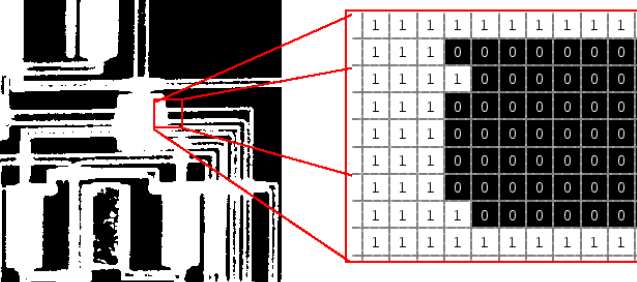
\includegraphics[scale=0.7]{Figures/2/binary-image}
			\caption{ภาพแบบ Binary }
			\label{Fig:binary-image }
		\end{figure}
		
		\item Grayscale Image เป็นรูปที่มี channel เดียว 
		โดยเก็บเป็นอาเรย์คล้ายกับภาพ Binary Image 
		แต่ค่าที่อยู่ในอาเรย์เป็นค่าความสว่าง ซึ่งมีค่าได้ตั้งงแต่ 0 ถึง 255
		ดังรูปที่ \ref{Fig:grayscale-image }
		\begin{figure}[H]
			\centering
			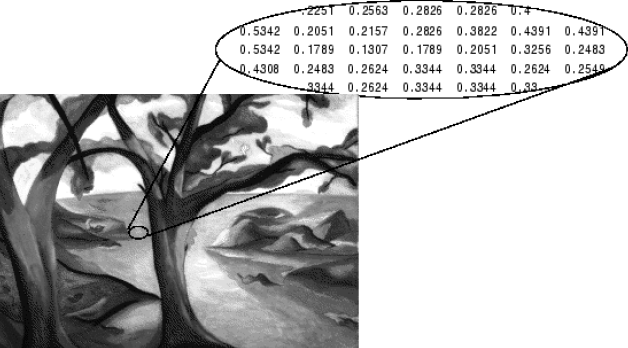
\includegraphics[scale=0.7]{Figures/2/grayscale-image}
			\caption{ ภาพแบบ Grayscale }
			\label{Fig:grayscale-image }
		\end{figure}
		
		\item RGB Image เป็นรูปที่มี 3 channel 
		โดยภาพจะเก็บอยู่ในรูปภาพโดเรียงตามลำดับ BGR 
		แต่ถ้าอยู่ในไฟล์ภาพจะเรียงตามปกติ คือ RBG 
		ดังรูปที่ \ref{Fig:rbg-image }
		\begin{figure}[H]
			\centering
			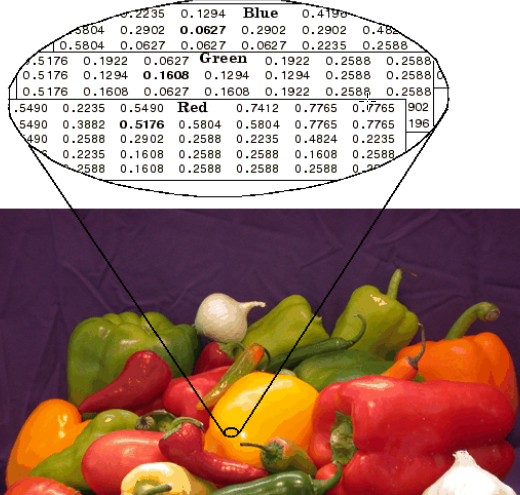
\includegraphics[scale=0.7]{Figures/2/rbg-image}
			\caption{ภาพแบบ RBG }
			\label{Fig:rbg-image }
		\end{figure}
	\end{itemize}

	\subsection{การทำ Thresholding รูปภาพ}
		การทำ Thresholding เป็นวิธีการแยกบริเวณรูปภาพ (Image Segmentation) ของภาพสีเทา (Grayscale) 
		จากรูปที่ \ref{Fig:thresholding} ผู้พัฒนากำหนดค่า threshold เท่ากับ 120 
		ในรูปภาพค่าพิกเซลแต่ละพิกเซลของภาพต้นฉบับที่มีค่าน้อยกว่า 120 
		จะถูกกำหนดเป็นค่าพิกเซลของภาพผลลัพธ์เป็น 0 (สีขาว) และถ้าในรูปภาพค่าพิกเซลแต่ละพิกเซลของภาพต้นฉบับนั้นมีค่ามากกว่าเท่ากับ 120 จะถูกกำหนดพิกเซลของภาพผลลัพต์เป็น 255 (สีดำ) จะได้สมการดังรูปที่  เมื่อ f(x, y) คือ ตำแหน่งพิกเซลของภาพต้นฉบับ และ g(x, y) คือ ตำแหน่งพิกเซลของภาพผลลัพธ์

		ตัวอย่างการทำ Thresholding ได้แก่การรูปภาพต้นฉบับนำมาเข้าสมการตามรูปที่ \ref{Fig:thresholding-example} และกำหนดค่า threshold เท่ากับ 120 ดังนั้นผลลัพธ์จะได้ดังรูปที่ \ref{Fig:thresholding-result}
		
		\begin{figure}[H]	
			\centering			
			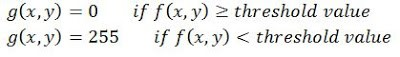
\includegraphics[scale=1]{Figures/2/thresholding}
			\caption{สมการการทำ Thresholding รูปภาพ}
			\label{Fig:thresholding}
		\end{figure}
		
		\begin{figure}[H]	
			\centering			
			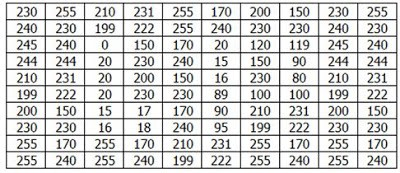
\includegraphics[scale=1]{Figures/2/thresholding-example}
			\caption{ตัวอย่างการทำ Thresholding รูปภาพต้นฉบับขนาด 10x10 พิกเซล}
			\label{Fig:thresholding-example}
		\end{figure}

		\begin{figure}[H]
			\centering					
			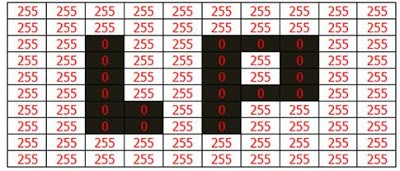
\includegraphics[scale=1]{Figures/2/thresholding-result}
			\caption{ตัวอย่างการทำ Thresholding รูปภาพผลลัพธ์ขนาด 10x10 พิกเซล}
			\label{Fig:thresholding-result}
		\end{figure}

	\subsection{การตรวจหา Canny Edge}
		การหาขอบภาพเป็นการหาเส้นรอบวัถตุที่อยู่ในภาพ เมื่อทราบเส้นรอบวัตถุจะสามารถคำนวณหาพื้นที่หรือจำแนกชนิดของวัถตุนั้นได้ ขอบภาพเกิดจากความแตกต่างของความเข้มแสงจากจุดหนึ่งไปยังอีกจุดหนึ่ง การตรวจหา Canny Edge [5] เป็นอัลกอริทึมการตรวจหาขอบที่เป็นที่นิยม ได้รับการพัฒนาโดย John F. Canny เป็นอัลกอริทึมแบบหลายขั้นตอนและจะดำเนินการผ่านแต่ละขั้นตอน
		\subsubsection{ลดสัญญาณรบกวน (Noise Reduction)} 
		เนื่องจากการตรวจหาขอบมีความอ่อนไหวต่อสัญญาณรบกวนในภาพ ขั้นตอนแรกคือการขจัดสัญญาณรบกวนด้วยตัวกรองแบบเกาส์ (Gaussian) 5x5 
		\subsubsection{การหาการไล่ระดับสีความเข้มของภาพ (Gradient)}
		รูปที่ Smoothing จะถูกกรองด้วย Sobel kernel ทั้งในแนวนอนและแนวตั้งจากจุดหนึ่งไปยังอีกจุด โดยการหาจุดในแนวนอน (Gx) และในแนวตั้ง (Gy) จากทั้งสอง ภาพนี้สามารถหาการไล่ระดับสีและทิศทางของขอบสำหรับแต่ละพิกเซล
		\subsubsection{Nonmaxima Suppression}
		หลังจากที่ผ่านขั้นตอนแรกมาแล้ว รูปที่ได้อาจจะมีเส้นขอบที่ไม่ใช่ขอบที่แท้จริงปรากฏอยู่ เนื่องจากสัญญาณรบกวนหรือลักษณะของวัตถุในภาพเป็นพื้นผิวที่มีลวดลายหรือมีรายละเอียดภายในมาก ดังนั้นเพื่อลดปัญหาดังกล่าวจึงได้มีการกำหนดค่า threshold ขึ้นมา 2 ค่า คือ High threshold (T1) และ Low threshold (T2) โดยพิกเซลที่มีค่ามากกว่า T1 จะถูกปรับเป็น 1 (ให้เป็นพิกเซลที่เป็นขอบ) แต่ถ้าน้อยกว่า T2 จะถูกปรับเป็น 0 ส่วนค่าที่อยู่ระหว่างค่า threshold ทั้งสอง การปรับเป็นค่า 0 หรือ 1 ขึ้นอยู่กับพิกเซลที่อยู่รอบข้าง หากพบว่าพิกเซลที่อยู่รอบข้างของพิกเซลที่เป็นขอบมีค่ามากกว่า T2 แล้ว จะปรับค่าพิกเซลดังกล่างให้มีค่าเป็น 1 และถือเป็นสมาชิกหนึ่งในภาพขอบด้วย
		\begin{figure}[H]
			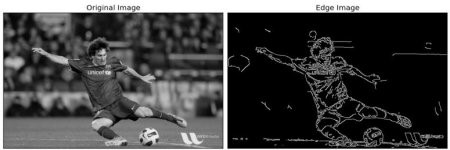
\includegraphics[width=\columnwidth]{Figures/2/canny-edge-detected}
			\caption{ตัวอย่างการตราจหา Canny Edge}
			\label{Fig:canny-edge-detected}
		\end{figure}


	\subsection{การหา Contour Approximation}
		\vspace{-5mm}

		รูปทรง (Contours) สามารถอธิบายได้ง่ายๆว่าเป็นเส้นโค้งที่เชื่อมต่อกับจุดต่อเนื่องทั้งหมดตามแนวขอบที่มีสีเดียวกัน และรูปทรงเป็นเครื่องมือที่มีประโยชน์สำหรับการวิเคราะห์รูปทรง การตรวจจับวัถตุและการจดจำ
		\vspace{-5mm}
		
		การใช้ภาพไบนารีจะได้ผลลัพธ์ที่มีความถูกต้องที่ดีกว่า ดังนั้นก่อนที่จะหารูปทรงควรใช้ threshold และ canny edge จากภาพก่อน ใน OpenCV การหารูปทรงคือการหาวัตถุสีขาวจากพื้นหลังสีดำ ดังนั้นวัถตุที่จะตรวจจับควรเป็นสีขาวและพื้นหลังควรเป็นสีดำ
		
		\begin{figure}[H]
			{\setstretch{1.0}\begin{lstlisting}
import  numpy  as  np  2   
import  cv2  im  =  cv2.imread('test.jpg')  
imgray  =  cv2.cvtColor(im,  cv2.COLOR_BGR2GRAY)  
ret,  thresh  =  cv2.threshold(imgray,  127,  255,  0)  
im2,  contours,  hierarchy  =  cv2.findContours(thresh,  cv2.RETR_TREE,  cv2.CHAIN_APPROX_NONE)  
			\end{lstlisting}}
			\caption{ตัวอย่างการใช้งานฟังก์ชัน cv2.findContours() โดยกำหนดค่าพารามิเตอร์เป็น cv2.CHAIN{\_}APPROW{\_}NONE}
			\label{Fig:finContoursNONE}
		\end{figure}
		\begin{figure}[H]
			{\setstretch{1.0}\begin{lstlisting}
import  numpy  as  np  2   
import  cv2  im  =  cv2.imread('test.jpg')  
imgray  =  cv2.cvtColor(im,  cv2.COLOR_BGR2GRAY)  
ret,  thresh  =  cv2.threshold(imgray,  127,  255,  0)  
im2,  contours,  hierarchy  =  cv2.findContours(thresh,  cv2.RETR_TREE,  cv2.CHAIN_APPROX_SIMPLE)  
			\end{lstlisting}}
			\caption{ตัวอย่างการใช้งานฟังก์ชัน cv2.findContours() โดยกำหนดค่าพารามิเตอร์เป็น cv2.CHAIN{\_}APPROW{\_}SIMPLE }
			\label{Fig:finContoursSIMPLE}
		\end{figure}
		
		จากรูปที่ \ref{Fig:finContoursNONE} ในการใช้ฟังก์ชัน cv2.findContours() 
		โดยกำหนดค่าพารามิเตอร์เป็น cv2.CHAIN{\_}APPROX{\_}NONE} จุดขอบทั้งหมดจะทุกเก็บไว้ 
		ซึ่งแตกต่างจากรูปที่ \ref{Fig:finContoursSIMPLE} ที่กำหนดค่าพารามิเตอร์เป็น cv2.CHAIN{\_}APPROW{\_}SIMPLE 
		จะทำการลบจุดที่ซ้ำซ้อนทั้งหมดและบีบอัดเส้นขอบทำให้ประหยัดหน่วยความจำ 
		และจากรูปที่ \ref{Fig:chain_approx_none_vs_simple} รูปสี่เหลี่ยมผืนผ้าแสดงให้เห็นถึงเทคนิคนี้ 
		เพียงวาดจุดบนพิกัดทั้งหมดในอาร์เรย์เส้น (เส้นสีน้ำเงิน)
		
		จากรูปที่ \ref{Fig:chain_approx_none_vs_simple} ภาพด้านซ้ายกำหนดค่าพารามิเตอร์เป็น 
		cv2.CHAIN{\_}APPROW{\_}NONE  ได้ทั้งหมด 734 จุด 
		และภาพด้านขวากำหนดค่าพารามิเตอร์เป็น cv2.CHAIN{\_}APPROW{\_}SIMPLE 
		ได้ทั้งหมด 4 จุด นั้นเป็นเหตุผลที่ผู้พัฒนาจะเลือกใช้ 
		cv2.CHAIN{\_}APPROW{\_}SIMPLE แทน cv2.CHAIN{\_}APPROW{\_}NONE เพื่อความประหยัดหน่วยความจำ

		\begin{figure}[H]
			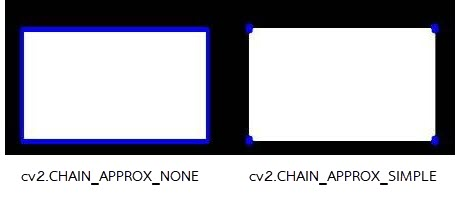
\includegraphics[width=\columnwidth]{Figures/2/chain_approx_none_vs_simple}
			\caption{ผลลัพธ์ของการหา Contours}
			\label{Fig:chain_approx_none_vs_simple}
		\end{figure}
	
	
	\subsection{Support Vector Machines (SVM)}
	SVM เป็นอัลกอริทึมในการคัดแยกที่มีการนำมาใช้กันในด้านการประมวลผลเป็นดิจิตอล 
	หลักการของ SVM คือการให้อินพุทที่ใช้ฝึกเป็นเวคเตอร์ในสเปซ N มิติ เช่นถ้าในกรณีของ 2 มิติ และ 3 มิติ 
	จะเป็นจุดที่อยู่ในระนาบ XY และ XYZ ตามลำดับ จากนั้นทำการสร้างไฮเปอร์เพลน (Hyperplane) 
	ที่จะแยกกลุ่มของเวคเตอร์อินพุทออกเป็นประเภทต่างๆ ในกรณีที่เป็น 2 มิติและ 3 มิติ ไฮเปอร์เพลน คือเส้นตรงและระนาบ 
	
	\begin{figure}[H]
		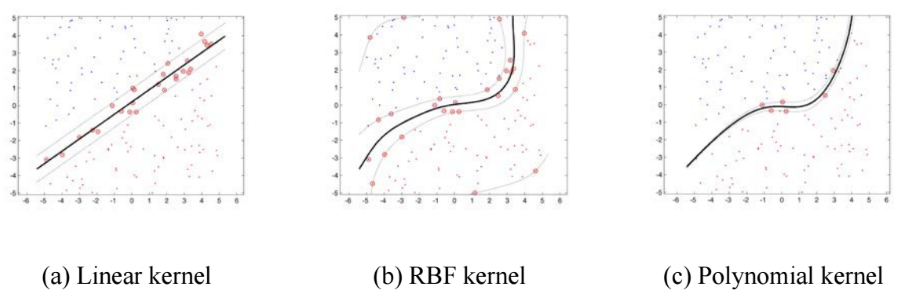
\includegraphics[width=\columnwidth]{Figures/2/format-kernel-function}
		\caption{รูปแบบ kernel function ในแบบต่างๆ}
		\label{Fig:format-kernel-function}
	\end{figure}

	ไฮเปอร์เพลนที่ได้จากการเลือกใช้ kernel function ที่ต่างกันก็จะให้ประสิทธืภาพการทำงานของโมเดลที่ต่างกัน นอกจาการเลือกใช้ kernel function ที่เหมาะสมแล้ว การกำหนดค่าต่างๆ (initial parameters) ของ kernel function ก็มีผลด้วยเช่นกันจากไฮเปอร์เพลนที่แสดงในรูปข้างบนเกิดจากการกำหนดค่าของ initial parameter ที่ต่างกันดังรูปที่ \ref{Fig:format-kernel-function}


	\subsection{K-Nearest Neighbour Algorithm }
	K-Nearest Neighbour Algorithm (KNN) [18] เป็นวิธีที่ใช้ในการจัดแบ่งคลาส (Classification) มีลักษณะการทำงานแบบ Supervised learing (ข้อมูลที่นำมาเรียนรู้ต้องมีคลาสกำกับไว้แล้ว) โดยเทคนิคนี้จะตัดสินใจว่า คลาสใดที่จะแทนเงื่อนไขหรือกรณีใหม่ๆ ได้บ้าง โดยการตรวจสอบจำนวนบางจำนวน (“K” ในขั้นตอนวิธีการ kNN) ของกรณีหรือเงื่อนไขที่เหมือนกันหรือใกล้เคียงกันมากที่สุด โดยจะหาผลรวม (Count Up) ของจำนวนเงื่อนไข หรือกรณีต่างๆ สำหรับแต่ละคลาส และกำหนดเงื่อนไขใหม่ๆ ให้คลาสที่เหมือนกันกับคลาสที่ใกล้เคียงกันมากที่สุด
	
	\subsubsection{ขั้นตอนวิธีการดำเนินการของอัลกอริทึมแบบ K-Nearest Neighbour Algorithm มีดังนี้}
	\begin{enumerate}
		\item กำหนดขนาดของค่า K 
		\item คำนวณระยะห่าง (Distance) ของข้อมูลที่ต้องการพิจารณากับกลุ่มข้อมูลตัวอย่าง
		\item จัดเรียงลำดับของระยะห่าง และเลือกพิจารณาชุดข้อมูลที่ใกล้จุดที่ต้องการพิจารณาตามจำนวนของค่า K ที่กำหนดไว้
		\item พิจารณาข้อมูลจำนวน K ชุด และสังเกตกลุ่มคลาสที่มีจุดใกล้กับจุดพิจารณาเป็นจำนวนมากที่สุด
		\item กำหนดคลาสให้กับจุดพิจารณาที่ใกล้จุดพิจารณมากที่สุด
	\end{enumerate}

	\subsubsection{การดำเนินการหลักของอัลกอริทึมแบบ K-Nearest Neighbour Algorithm ประกอบไปด้วยการทำงาน 2 ฟังก์ชัน ได้แก่}

	\begin{enumerate}
		\item ฟังก์ชันระยะทาง (Distance Function) เป็นการคำนวณค่าระยะห่างระหว่างสองจุด เพื่อที่นำมาวัดความคล้ายคลึงของข้อมูล
		\item ฟังก์ชันการแจกแจง (Combination Function) เป็นการรวมกันของผลลัพธ์ที่ได้จากการคำนวณค่าระยะห่างโดยทำการเรียงลำดับค่าระยะห่างจากน้อยไปมาก จากนั้นนำมาเปรียบเทียบกับค่า K เพื่อหาคลาสของเป้าหมาย
	\end{enumerate}

	\subsection{Random Forest Classifier }
	Random Forest Classifier (RFC) [19] เป็นวิธีที่ใช้ในการจัดแบ่งคลาส โดยหลักการสุ่มข้อมูล (Random sampling) เพื่อสร้างต้นไม้ตัดสินใจขึ้นมาจำนวนมาก ในการจำแนกคลาสของวัถตุโดยจะอินพุทข้อมูลเวกเตอร์ (Vecter) ใส่ให้แต่ละต้นไม้ตัดสินใจที่ถูกสร้างขึ้นมา ต้นไม้แต่ละต้นจะให้คะแนนสำหรับข้อมูลเวกเตอร์ที่ถูกป้อนเข้ามาในแต่ละคลาส วิธีการ Random Forest จะเลือกคลาสที่มีคะแนนมากที่สุดและทำนายคลาสของวัถตุ


\section{การหาขนาดของยาด้วยการใช้วัถตุอ้างอิง}
	การหาขนาดยาด้วยการใช้วัถตุอ้างอิง ด้วยวิธีการเทียบบัญญติไตรยางศ์ [20] เนื่องจากรูปภาพมีหน่วยเป็นพิกเซลและรู้ขนาดด้านยาวและกว้างของวัถตุอ้างอิงแล้ว ถ้าหากวัตถุอ้างอิงมีขนาดด้านยาวเท่ากับ 15 เซนติเมตร ขนาดด้านกว้างเท่ากับ 10 เซนติเมตร และวัตถุอ้างอิงในรูปที่ตรวจจับได้ด้วยการหา Contours ได้ขนาดด้านยาวเท่ากับ 98 พิกเซล ขนาดด้านยาวเท่ากับ 65 พิกเซล และขนาด 1 พิกเซล จะเท่ากับกี่เซนติเมตร ด้วยการเทียบบัญญติไตรยางศ์ จะได้ว่า 15 (เซนติเมตร) / 98 (พิกเซล) เท่ากับอัตราส่วน 0.153 เซนติเมตร/พิกเซล ดังนั้น 1 พิกเซล จะเท่ากับ 0.153 เซนติเมตร และสามารถหาขนาดของยาด้วยการนำ 0.153 ไปคูณกับขนาดพิกเซลของรูปภาพยา

\section{เครื่องมือที่ใช้ในการพัฒนา}
	Nginx [8] มาจากคำว่า “Engine-X” เป็นเว็บเซิร์ฟเวอร์ที่มีประสิทธีภาพดีและนิยมอยู่ในปัจจุบัน ถูกคิดค้นขึ้นมาเพื่อให้สามารถที่จะรองรับการทำงานได้มากกว่า Apache[6] และนอกจากนี้ Nginx ยังมีโมดูลเสริมเข้ามาที่เพียงพอต่อการใช้งานทั่วไป และเป็นซอฟแวร์แบบ Open Source ที่สามารถใช้งานได้ฟรีโดยรองรับระบบปฏิบัติการ Linux และ ระบบปฏิบัติการ Windows
	
	MySQL [7] เป็นโปรแกรมจัดการฐานข้อมูลที่รองรับคำสั่ง SQL เป็นเครื่องมือสำหรับเก็บข้อมูล ที่ต้องใช้ร่วมกับเครื่องมือหรือโปรแกรมอื่นอย่างบูรณาการ เพื่อให้ได้ระบบงานที่รองรับความต้องการของผู้ใช้ เป็นฐานข้อมูลเชิงสัมพันธ์ (RDBMS) ผู้พัฒนาได้นำมาใช้งานกับเว็บเซอร์วิสในการจัดเก็บฐานข้อมูลการพิสูจน์เอกลักษณ์ยาเม็ดหรือแคปซูล
	
	Express – Node.js [3] ถูกสร้างขึ้นบนฐานของระบบ Node.js ซึ่งมีความเร็วของการทำงานและมีความครบถ้วนของระบบ ครอบคลุมในส่วนของการทำงานพื้นฐานในการทำเว็บเซอร์วิส ใช้ในการทำ routing[2] middleware การจัดการ request และ response ทื่ถูกส่งมาจากแอปพลิเคชัน

